\documentclass[10pt]{article}

\usepackage{lipsum}
\usepackage{graphicx}
\usepackage{amsmath}
\usepackage{hyperref}

\usepackage[section]{placeins}

\usepackage{etoolbox}
\usepackage[onehalfspacing]{setspace}
\AtBeginEnvironment{figure}{\singlespacing}
\AtBeginEnvironment{table}{\singlespacing}

\usepackage{caption}
\DeclareCaptionFont{8pt}{\fontsize{8pt}{9pt}\selectfont}
\captionsetup{font={8pt}}


\usepackage[
	backend=biber,
    style=authoryear,
	url=false,
    %sorting=ynt,
    bibwarn=true,
    bibencoding=utf8,
	uniquename=false,
    sortlocale=de_DE,
    maxbibnames=99,
    maxcitenames=2]{biblatex}
\renewbibmacro{in:}{}
    
\DefineBibliographyStrings{english}{
   andothers = {{et\,al\adddot}},}
   
\addbibresource{../../../bib/thesis.bib}

\AtBeginEnvironment{figure}{\singlespacing}
\AtBeginEnvironment{table}{\singlespacing}


\begin{document}


\begin{titlepage}
	\centering
	{\scshape\LARGE Ludwig-Maximilians-Universität München \par}
	{\scshape\large Faculty of Biology, Computational Neuroscience \par}
	\vspace{0.5cm}
	\includegraphics[width=0.4\textwidth]{../logo/siegel_black.pdf}\par
	\includegraphics[width=0.7\textwidth]{../logo/GSN-Logo_ab35mmBreite_RGB.jpg}\par
	\vspace{0.7cm}
	{\scshape\LARGE Master's Thesis \par}
	\vspace{0.05cm}
	\vspace{0.05cm}
	{\huge\bfseries Computational Simulation of Time Perception \par}
	\vspace{1.4cm}
	{\Large Katharina \textsc{M Bracher} \par}
	%{Student ID: 11754625 \par}
	\vspace{0.5cm}
	{\large Supervision: Dr. Kay \textsc{Thurley} \par}
	{\large Prof. Dr. Andreas \textsc{Herz} \par}
\end{titlepage}


\normalsize
\tableofcontents

%\the\textwidth 
%\makeatletter\f@size
% 345 pt = 4.79167 in -> figures 4.75 in 
% text 10 pt, fig caption 8 pt
% in drawio 10 pt -> 13.3; 8 pt -> 10.66 
\pagebreak


\section{Introduction}
%---> behavior, predictive coding/updates, noise
Animals are able to produce complex and flexible behaviors that often rely on the interplay of motor and sensory systems.
%internal models in motor control
To guide behavior, animals are thought deploy predictive internal signaling, allowing the animal to contemplate sensory consequences. 
In this sense the CNS uses intrinsic neural representations of motor actions and both control and prediction to achieve desired or expected sensory consequences \cite{Straka2018}.
If there is a mismatch in predicted and actual sensory feedback, the internal model is updated by an error signal. 

Externally-derived inputs, however, are subject to noise that arises from the variability of the environment. An additional source of noise is neural representation of the input.
Thus, sensory inputs need to be constantly processed and combined with prior expectations.
Magnitude estimation involves establishing a relationship between external events and their perception by e.g. evaluating or reproducing a stimulus. Therefore, magnitude estimation is useful to explore sensory processing. 
A variety of experimental studies have found characteristic behavioral effects on magnitude estimation across sensory modalities (\cite{Petzschner2015}).

\subsection{Behavioral Effects in Magnitude Estimation}
%---> magnitude estimation, optimization, bayes
The most prominent observation in stimulus reproduction is a regression to the mean of stimuli, i.e. small stimuli are overestimated whereas large stimuli are underestimated (\textit{regression effect}). 
This effect intensifies for ranges with larger stimuli (\textit{range effect}).
For larger stimuli the standard deviation of estimates increases monotonically (\textit{scalar variability}). 
Finally, the recent history of stimuli presentations influences the current stimuli estimation (\textit{sequential effects}).
All effects mentioned above are displayed in Fig. \ref{fig:behavioraleffects}. 
Modality-independence of these effects suggests the existence of a common underlying principle or processing mechanisms, that would explain e.g. an optimal strategy for unreliable judgments due to noise.
Minimizing errors in judgment can be achieved by integrating prior experience with immediate sensory input and is therefore often described with Bayesian models.
In Bayesian models sensory information is represented by a likelihood function is combined with prior experience (prior distribution) that together result in biased estimates (posterior distribution).
%Interaction between immediate and prior experience is likely used to minimize errors and is therefore often described with Bayesian models.

\begin{figure}[ht]
	\centering
	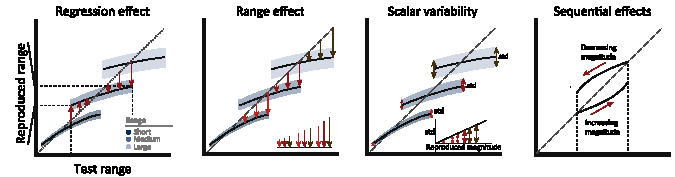
\includegraphics[width=\textwidth]{figures/behavioural_effects_petzschner.pdf}
	\caption{\textbf{Behavioral effects.} 
	\textit{Regression effect}: in a range of stimuli large stimuli are underestimated, and small stimuli are overestimated which results in a regression to the mean of the range.
	\textit{Range effect}: the regression to the mean gets more pronounced for ranges that comprise larger stimuli. 
	\textit{Scalar variability}: the standard deviation of the reproduced magnitude grows linearly with larger rages. 
	\textit{Sequential effects}: the history presented stimuli (e.g. ascending or descending order) has an influence on the reproduced magnitude. 
	Adapted from \cite{Petzschner2015}.}
	\label{fig:behavioraleffects}
\end{figure}


\subsection{working title: Neural Correlates of Timing}
%---> timing, time reproduction experiments, methods to measure time
Timing, as an example of magnitude estimation, is a critical ability for anticipating and coordinating interactions with the environment. 
Experiments in which subjects have to measure and reproduce time intervals, can be used to study how the brain integrates information from the past with current sensory input in order to achieve correct timing.
Time reproduction is usually accomplished by one or more measurement periods in which the temporal stimulus is presented, and a reproduction period that is terminated by movement initiation from the subject.
Time between two events can be measured in an absolute or predictive manner. In the case of absolute timing, time can be continuously estimated from an output that results from integration of ticks from a central clock  The rate at which activity increases does not depend on the time interval. In contrast, in predictive timing a fixed state is reached at the end of the time interval, by adjusting the rate of increase according to the anticipated time. 

%---> nerual implementation, brain ares, scaling, trajectories, speed command, motor simulationk error signal
To measure and produce time intervals, flexible control of neural mechanisms is required. 
A brain area that has been associated with timing behavior is the medial prefrontal cortex (MFC) (\cite{Wang2018}, \cite{Emmons2017}, \cite{Genovesio2006}, \cite{Lewis2004}, \cite{Shima2000}).
Single cell activity shows heterogeneous response profiles, but often temporally scaled according to produced time intervals (\cite{Henke2021}, \cite{Sohn2019}, \cite{Wang2018}).
Scaling is a phenomenon that consistent at the population level. Population activity can be displayed in a low-dimensional state space, where the activity by all neurons is represented over time by a so-called neural trajectory.
Activity at the level of neural populations displays characteristic trajectories in the state space (\cite{Henke2021}, \cite{Meirhaeghe2021}, \cite{Sohn2019}, \cite{Wang2018}). 

%%%%%%%%%%%%%%%
For time interval reproduction, neural trajectories have been shown to evolve to a fixed state. The speed of the neural trajectory is inversely proportional to the time interval.
The neural trajectories are consistently influenced by prior beliefs.
It has been shown, that flexible motor timing can be achieved by controlling the speed of neural dynamics (\cite{Sohn2019}, \cite{Wang2018}). 
%to minimize prediction error, where the prediction errors signal mismatches between predicted input and the input actually received
%feedback used to update estimates. 
%Work in multiple modalities has provided support for a hypothesis that neural activity can be understood at the level of neural populations and viewed as neural trajectories of a dynamical system
%scaling
Further, it has been found that neural activity in anticipation of a delayed response reaches a fixed threshold with a rate inversely proportional to delay period (\cite{Murakami2014}, \cite{Mita2009}).
%error signal, update

%---> Curcuit model, decition making, elements
%model used only for... in secific task
%Here, we aimed to answer this question using a dynamical systems approach. 
\cite{Wang2018} proposed a potential neural mechanism for speed control. Based on that mechanism \cite{Egger2020} developed an extended circuit model for sensorimotor timing.

%---> research questions
%can the model be applied to experiment simulations? it was only fitted to data separatly. can the model be applied to more realistic experiment simulations?
%does the model in experiment simulations exhibit typical effects of magnitude estimation? How much of the effects in real behavior does it capture?
%are there other predictions the model does? variance; andere effecte ranges

\section{Model Description}
Flexible speed control can be achieved by a simple model consisting of three units, $u, v, y$ that represent population activity. 
\subsection{Basic Circuit}
The dynamics of $u, v$, and $y$ are defined as follows:
\begin{equation} \label{circuit}
	\begin{split}
	\tau\frac{\text{d}u}{\text{d}t} & = -u + \theta(W_{uI}I - W_{uv}v + \eta_u) \;, \\
	\tau\frac{\text{d}v}{\text{d}t} & = -v + \theta(W_{vI}I - W_{vu}v + \eta_v) \;, \\
	\tau\frac{\text{d}y}{\text{d}t} & = -y + W_{yu}u - W_{yv}v + \eta_y \;.
	\end{split}
\end{equation}
Two units, $u$ and $v$, receive a tonic symmetric input $I$ ($W_{uI}=W_{vI}=6$) and are mutually inhibiting each other ($W_{uv}=W_{vu}=6$). 
The inputs to $u$ and $v$ are governed by a sigmoid activation function $\theta(x) = \frac{1}{1+exp(-x)}$.
The output unit $y$ receives excitatory input from $u$ and inhibitory input from $v$ ($W_{yu}=W_{yv}=1$) which results in a ramp-like activity of $y$.
All three units have a time constant $\tau = 100$~ms. 
Stochastic synaptic inputs are modeled as independent white noise $\eta_u, \eta_v, \eta_y$ with standard deviation $\sigma$.
Initial conditions of $u, v$ and $y$ have been optimized for in \cite{Egger2020} and are set to $u_0=0.7, v_0=0.2, y_0=0.5$ (Fig. \ref{fig:circuit}a)

Depending on the input $I$, the system shows different dynamics. For low levels of $I$ (0$<$I$<$0.5) the system has three fixed points (two stable, one unstable at $u=v$) and $y$ ramps up faster the higher input $I$. 
For intermediate values of $I$ (0.5$<$I$<$1) the system still shows three fixed points of the same sort as in the low input regime (Fig. \ref{fig:circuit}b)but $y$ ramps up with a slope that is inversely proportional to the input $I$ ($y$ ramps up slower the higher input $I$, see Fig. \ref{fig:circuit}c). 
For high $I$ (1$<$I) the system has one stable fixed point (at $u=v$) and $y$ ramps down faster for higher $I$.
Thus, the speed at which the output $y$ evolves can be controlled by the input $I$ (Fig. \ref{fig:circuit}d) and determines the time interval after which $y$ reaches a fixed threshold $y_{\text{th}}$. 
In interval reproduction experiments, reaching a threshold $y_{\text{th}}$ can be understood as movement initiation time, which can be controlled for by adjusting $I$.
In this report, the intermediate input regime is explored: higher inputs result in a shallower slope of $y$, such that the threshold $y_{\text{th}}$ is reached after a longer time interval.

%%%%%%%%%%%%%%%%%%%%%%%%%%%%%%%%%%%%%%%%%%%%%%%%%%%%%%%%%%%%%%%%%%%% nullcline
\begin{figure}[ht]
	\centering
	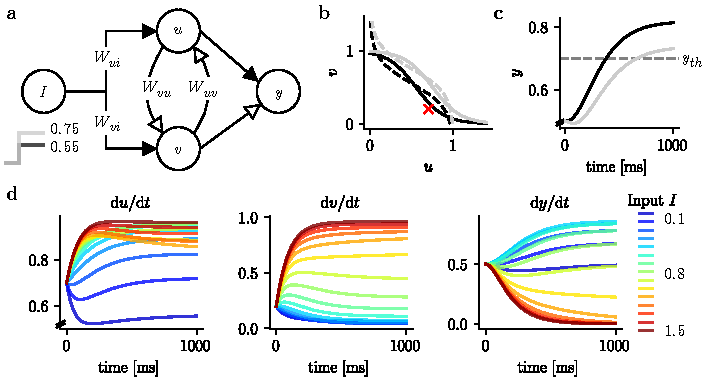
\includegraphics{figures/defCircuit_nullcl.pdf}
	\caption{\textbf{Basic circuit and input regimes.} 
	\textbf{(a)} $u$ and $v$ share a common input $I$. The input is governed by weights $W_{uI}$ and $W_{vI}$. The two units have reciprocal inhibitory connections, with weights $W_{uv}$ and $W_{vu}$ that determine the inhibitory strength. Both project to the output unit $y$ with an excitatory connection from $u$ and an inhibitory connection from $v$. Excitatory and inhibitory connections are shown by filled and open arrows, respectively. 
	\textbf{(b)} The control of the speed in $y$ can be analyzed in the phase plane of $u$ and $v$. The $u$ (dashed) and $v$ nullcline (solid) is shifted when the input is increased from $I=0.65$ (black) to $I=0.75$ (gray). In the intermediate regime, the systems shows two stable and one unstable fixed point. The red cross indicates the initial conditions for the dynamics in (c). Depending on $I$, with the same initial conditions, the system evolves faster or slower to the stable fixed point. 
	\textbf{(c)} Dynamics of $y$ for intermediate regime with input $I=0.75$ in gray and $I=0.65$ in black. There is an inverse relation of input strength and slope. With higher input, the threshold at 0.7 (dashed line) is reached after a longer time interval. 
	\textbf{(d)} Dynamics of $u, v, y$ for inputs from $0.1\leq I \leq 1.5$ are shown. Initial conditions are set to $u_0=0.7, v_0=0.2, y_0=0.5$. With these initial conditions and values of $I>=0.5$, the relation of steady state activity of $y$ (and slope to reach the steady state) is inverse to $I$ (intermediate and high $I$ regime). For values $I<=1$ the activity of $y$ ramps down (yellow corresponds to $I=1$). For $I<0.5$ the steady state (slope) is smaller the smaller $I$ (low $I$ regime, dark blue).}
\label{fig:circuit}
\end{figure}

\subsection{Update Mechanism and Experiment Procedure}
Basic interval reproduction experiments can be designed with only two epochs: a measurement epoch that has the duration of the stimulus interval and a reproduction epoch that starts immediately after the measurement epoch (Fig. \ref{fig:epochs}b). 
The basic circuit described above is modified to perform interval reproduction (see Figure \ref{fig:epochs}a for schematic of modified circuit).
The relation of input $I$ with the slope of the ramping activity of $y$ is used in combination with a fixed threshold $y_{\text{th}}$.
By adding an update mechanism that flexibly adjusts $I$, the threshold crossing of $y$ can be delayed or moved to earlier times.
This way, measuring and reproducing an interval is done predictively, by adjusting the slope of the ramp such that the output reaches the threshold after the intended time.
%In other scenarios, time could be encoded by the level a ramp reaches with a fixed slope.
In the model the measurement epoch is fixed to the stimulus interval $t_s$, and the reproduction epoch ends, when $y$ reaches the fixed threshold $y_{\text{th}}$ from below. 
The time from the end of the measurement epoch until the threshold-crossing of $y$ yields the reproduced time interval $t_r$ that is aimed to equal the stimulus interval $t_s$ (Fig. \ref{fig:epochs}c).

\begin{figure}
	\centering
	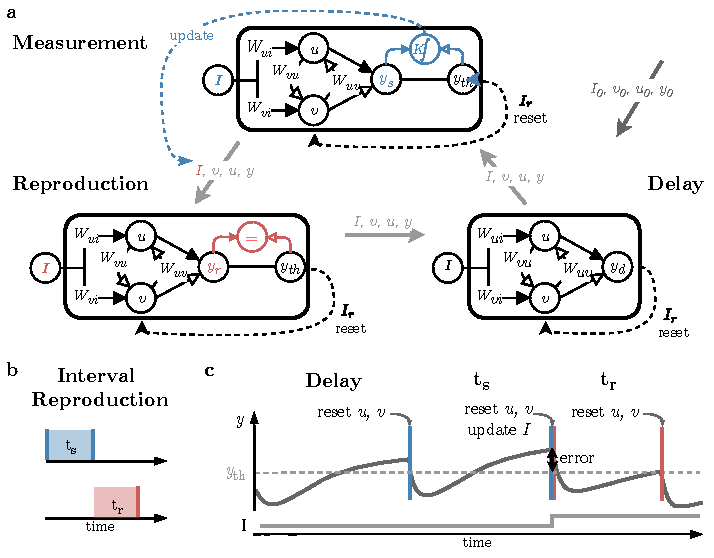
\includegraphics{figures/epochs.pdf}
	\caption{\textbf{Extended circuit for experiment simulation.} 
	\textbf{(a)} The circuits for measurement, reproduction and delay epoch are displayed. All circuits comprise the same basic structure with different additional elements that are unique for the epoch. Initial values of $u, v, y$ and $I$ are fed into the delay circuit for the duration of the initial interval. $u$ and $v$ are reset with a transient input $I_r$ before end values of $u, v, y$ and $I$ are transferred to the measurement circuit as new initial conditions. After the duration of the stimulus interval, the difference between $y$ and the threshold $y_{\text{th}}$ is used with the memory parameter $K$ to update $I$ together with another reset of $u$ and $v$. The values are transferred with all other variables to the reproduction circuit. The reproduction epoch ends when $y$ reaches the threshold $y_{\text{th}}$ from below. Before the presentation of another stimulus interval, there is again a delay period with no update of $I$. The reset mechanism enables the model to simulate an arbitrary number of stimulus intervals. Adapted from \cite{Egger2020}.
	\textbf{(b)} Interval reproduction experiment with stimulus interval $t_s$ (blue) and reproduction $t_r$ (red).
	\textbf{(c)} Schematic of one trial. After a delay epoch, $u$ and $v$ are reset. The measurement epoch lasts for the duration of the stimulus interval $t_s$. $y$ should reach the threshold $y_{\text{th}}$ (dashed line) at exactly the time the stimulus interval ends. The threshold was crossed well before the end of the interval and at the end of the measurement epoch, the error in $y_m$ to the threshold $y_{\text{th}}$ is used to update $I$. To reach the threshold at a later time, $I$ is increased, which reduces the slope of $y$ in the reproduction epoch. After the reset of $u$ and $y$ and the update of $I$ the reproduction ends when $y$ reaches the threshold. The time after the reset and update until the threshold crossing denotes the reproduced interval $t_r$.}
\label{fig:epochs}
\end{figure}

\noindent
 The following update mechanism of $I$ is based on the intermediate input regime, that shows an inverse relation of $I$ to the slope of $y$ (Fig. \ref{fig:circuit}b).
The error signal is determined at the end of the measurement epoch and is composed of the difference of $y$ to the threshold $y_{\text{th}}$.
If the threshold $y_{\text{th}}$ is not reached during the measurement epoch, the slope has to be adjusted, such that $y$ ramps up faster to reach the threshold at exactly the time of the stimulus interval. For a steeper slope, $I$ is reduced.
If $y$ crossed the threshold before the measurement epoch ends, so is above $y_{\text{th}}$ by the end of the stimulus interval, the slope needs to be reduced in order to reach the threshold at a later time in the reproduction. For a shallower slope, $I$ is increased (Fig. \ref{fig:epochs}c).
$I$ is adjusted according to the error $(y-y_{\text{th}})$, weighted by a memory parameter $K$ right at the end of the measurement epoch
\begin{equation} \label{Iupdate}
	\begin{split}
	\tau\frac{\text{d}I}{\text{d}t} & = sK(y-y_{\text{th}}) \;.
	\end{split}
\end{equation}
The update of $I$ is only active for a pulse between the measurement and reproduction epoch ($s=1$) and inactive for all other times ($s=0$).
Further, $u$ and $v$ receive a transient input pulse $I_r$ to reset the dynamics for the subsequent epoch (Fig. \ref{fig:epochs}c)
\begin{equation} \label{experimentcircuit}
	\begin{split}
	\tau\frac{\text{d}u}{\text{d}t} & = -u + \theta(W_{uI}I - W_{uv}v + \eta_u - I_r) \;,\\
	\tau\frac{\text{d}v}{\text{d}t} & = -v + \theta(W_{vI}I - W_{vu}v + \eta_v + I_r) \;.\\
	\end{split}
\end{equation}
Resetting the dynamics after the reproduction epoch enables the model to simulate an arbitrary number of stimulus intervals. 
Before a new stimulus presentation there is a delay period: at the beginning of an experiment with a sequence of stimuli there is an initial interval with the initial values of $u, v, y$ and an initial input $I_0$ (Fig. \ref{fig:epochs}c). 
This initial interval allows the model to get closer to steady-state before the stimulus presentation starts. 
Reproductions that do not reach the threshold in a certain time span  or too early are classified as timeout trial.
%sup

To simulate variability in the reproductions as it is found in real data, noise is added to $u, v$ and $y$ in the implementation. In data, a monotonic increase of the standard deviation of reproductions is found (\textit{scalar variability}). 
If noise levels in the model are too high ($\sigma>0.2$) the standard deviation of reproductions is not growing monotonically with $\sigma$ (\cite{Egger2020}).
For all simulations, $\sigma$ was set to 0.02, which results in a realistic coefficient of variation of 0.1 (Supplementary Fig. \ref{sup:CV}b, c).
%todo: cite plausible CV
In Figure \ref{fig:experiment}a five example trials and the activity of $u, v, y$ and $I$ are depicted. 
In the full simulation, 500 stimuli randomly chosen from a stimulus distribution were presented. The uniform distribution of time intervals is denoted as stimulus range. 
The stimulus range consisted of seven stimuli ranging from 400-700 ms (\ref{fig:experiment}b).

The experiment simulation results in a distribution of reproduced time intervals for each stimulus and a distribution of inputs that drive the activity of $y$ in the reproduction (Fig. \ref{fig:experiment}c).
Taking the mean over the distribution of reproduced time intervals for each stimulus allows for the investigation of effects in the behavioral results (Fig. \ref{fig:experiment}d). 

\begin{figure}[ht]
	\centering
	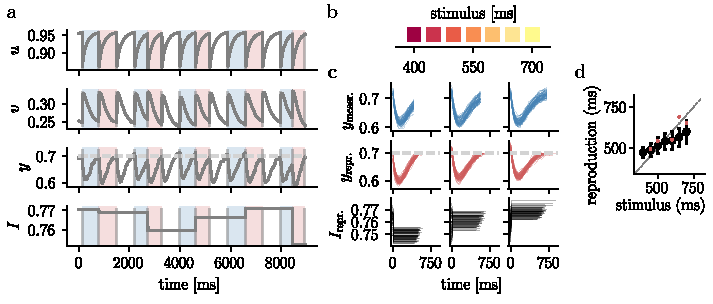
\includegraphics{figures/trial.pdf}
	\caption{\textbf{Experiment description.} 
	\textbf{(a)} The dynamics of $u, v, y $ and $I$ are displayed over time for five consecutive example trials (650, 500, 600, 700, 450 ms) of an experiment simulation with 500 trials. Stimulus presentation and reproduction epochs are highlighted in blue and red, respectively. Before new stimuli presentations, there is a 700 ms delay period (white). Initial values for the experiment simulation are set to $u_0=0.7, v_0=0.2, y_0=0.5, I_0=0.8$. The added noise is set to $\sigma=0.02$ and the memory parameter to $K=5$. The threshold is set to $y_{\text{th}}=0.7$ (dashed line). Reproduced times are 690, 540, 550, 650, 490 ms.
	\textbf{(b)} For the experiment, simulation time intervals were randomly drawn from a discrete, uniform stimulus distribution. The range of time intervals contained stimuli from 400 to 700 ms with steps of 50 ms.
	\textbf{(c)} The measurement (upper) and reproduction (middle) epoch of $y$ and input for reproduction (lower) are shown for the full experiment, sorted according to stimulus interval. Shown are trials for stimuli of 400, 550 and 700 ms (depicted above).
	\textbf{(d)} Mean reproduction and standard deviation (black) across trials for each stimulus interval of the experiment stimulation shown (c). If the mean lies on the identity line (dashed line), reproduction time corresponds to the stimulus interval on average. Red dots show the reproductions of the example trials shown in (a). 
	}
\label{fig:experiment}
\end{figure}

\section{Parameters in Accordance with Error Minimization}
We asked whether the behavioral effects observed in real data (Fig. \ref{fig:behavioraleffects}) could be reproduced by experiments with the circuit model, which itself is based on the scaling phenomenon found in brain data. 
A crucial value to adapt was the memory parameter $K$, since this parameter defines the weight with which the input is adjusted to compensate for the discrepancy between the predicted interval and the stimulus duration.
Another parameter that had to be considered is the time constant $\tau$, which affects how fast $y$ behaves in response to the input. Therefore, $\tau$ can be interpreted as a biophysical parameter of the model that describes the rate of a population.
In contrast to \cite{Egger2019}, parameters such as the initial values, especially $I_0$ did not need to be adjusted in advance. This is because the input will have settled after the first one or two trials and will not be affected by the initial values thereafter.
%weights 
%noise adjusted to plausible CV in results
In the following, the threshold was set to 0.7, but smaller and larger thresholds were tested as well.
For evaluating effects in behavior, two stimulus ranges were used in simulations, denoted as short and long range. The short range contained seven stimuli ranging from 400-700~ms. The long range also contained seven stimuli that were shifted up by 300~ms compared to the short range, ranging from 700-1000~ms.

 
\subsection{Behaviorally Plausible Slopes}
The regression effect in behavior can be quantified by the slope that results from a linear regression between the stimuli and the reproductions.
Biological plausible slopes lie around 0.83 for the short and 0.73 for the long range.
Interestingly, this is the case in across time domains, regardless of whether the short and long range are situated in the millisecond or second domain. (\cite{Thurley2018}, \cite{Jazayeri2010}). 
The slopes of behavioral results for multiple combinations of the update parameter~$K$ and the time constant~$\tau$ were determined. 
In broad parameter regimes, the reproductions show a regression to the mean, as indicated by a slope smaller than 1. 
For fixed $\tau$, the regression increases as $K$ increases, since more weight is given to the current update, and consequently less reliance is placed on the prior. 
The model also produced biological plausible slopes for different time constants (Fig. \ref{fig:parameter}a), where $K$ must be adjusted depending on the stimulus range and time constant. 
To produce plausible slopes, $K$ takes on smaller values for the long range, putting less weight on the update compared to the short range.

\subsection{Model Regime for Error-Minimized Behavior} %Parameters that Minimize Errors in Reproductions
Can behavioral effects of magnitude estimation also be achieved by adjusting $K$ and $\tau$ in accordance with error minimization?
To find such optimized parameters, the mean squared error was minimized, which is defined as the sum of the squared bias and variance of the mean reproductions (Supplementary Eq. \ref{MSE}).
For larger time constants~$\tau$, the optimized update parameter~$K$ increases. Values of $K$ that minimize errors are smaller for the long range compared to the short range for all $\tau$, as already found for values of $K$ that result in plausible slopes.
The corresponding time constant $\tau$ for the overall minimum of the MSE differ between the two stimulus ranges. For the short stimulus range, $\tau* = 120$ ms and $K* = 11$ yields an overall minimum, whereas $\tau* = 200$ ms, $K* = 20$ yields a overall minimum for the long range. 
Assuming the same rate time constant across experiments, we had to find a shared $\tau$ for both the short and long range. Consequently, a time constant between the optima was chosen, considering the overlap with biological plausible slopes. Only with a time constant of 130~ms, optimal $K$ coincided with biological plausible slopes in both ranges. 
With a time constant of $\tau = 130$, $K* = 13$ for the short and $K* = 10$ for the long range (Fig. \ref{fig:parameter}b, Supplementary Fig. \ref{sup:othererror}a, b).
Behavioral results with error-minimizing parameters show a regression to the mean with a stronger regression for the long range (slope of 0.73) compared to the short range (slope of 0.77) (Fig. \ref{fig:parameter}c). For dynamics of $y$ for single trials over the course of the experiment, see Supplementary Fig. \ref{sup:experiment}.
Adjusting $K$ in accordance with error minimization, leads to putting more weight on the prior experience for longer stimuli, which naturally entail more uncertainty, and is thus biological plausible.
The model produces behavior that shows the regression and the range effect.
Yet, the slope for the small range lies below the biological plausible slopes found in data. 
The standard variation of reproductions increases linearly (scalar variability), the mean coefficient of variation (CV) for the short range is 0.09, for the long range 0.11 (Fig. \ref{fig:parameter}c).
No range effect can be observed when minimizing the error in reproductions based on the squared bias or the variance instead of the MSE. The relation of stronger weighting of the prior for the long range due to decreased $K$ is not apparent for either error metrics (Supplementary Fig. \ref{sup:othererror}c, d).  
%supp

\begin{figure}[ht]
	\centering
	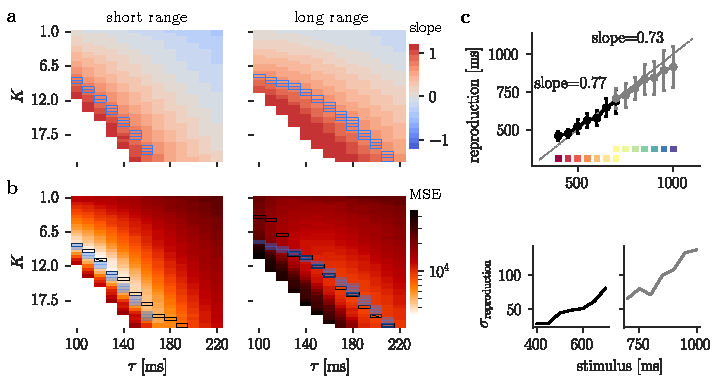
\includegraphics{figures/interIparams.pdf}
	\caption{\textbf{Behavioral effects and parameter optimization.} 
	\textbf{(a)} Simulations with 500 trials for each pair of memory parameter $K$ and time constant $\tau$ at noise level $\sigma = 0.02$. Simulations were performed with stimuli chosen from the short (left) or long range (right). Color scale represents the slope of the linear fit between stimuli and reproductions. A slope of 1 on the identity line corresponds to perfect reproduction of the stimuli. Behaviorally plausible slopes are encircled in blue and lie around 0.83 for the short and 0.73 for the long range. Empty space corresponds to simulations, that exceeded the number of timeout trials and were thus excluded from analysis.
	\textbf{(b)} Optimization of the weight given to the update $K$ for different time constants $\tau$ at noise level $\sigma = 0.02$. Color scale represents the MSE for an experiment stimulation with 500 trials for each pair of $K$ and $\tau$. Stimuli were either chosen from the short (left) or the long stimulus range. The minimal error for each $\tau$ is encircled in black and minimal error across all $\tau$ is additionally crossed. Parameter combinations that result in behaviorally plausible slopes (a) are shaded in blue.
	\textbf{(c)} Top: Mean reproductions for simulation with 500 trials for each stimulation with the short (black) and long (gray) stimulus range. The value of $K$ is optimized for a time constant of $\tau = 130$ ms. For the simulation with short stimulus range $K*$ was 13, with the long stimulus range optimal $K*$ was 10. 
		The slope is the result of a linear regression between stimuli and reproductions.
		Inset: For experiment simulations two stimuli ranges were used. The short range contained stimuli from 400 to 700 ms, the long range contained stimuli from 700 to 1000 ms.
		Bottom: Standard deviation of reproductions for each stimulus for the short and long range from the simulation in (c).
	}
\label{fig:parameter}
\end{figure}

\section{Comparison of Intermediate and High Input Regime}
There are differences between the intermediate and high input regimes in terms of fixed points and dynamics.
Nevertheless, simulations of time reproduction experiments are possible in both regimes. 
In the following, simulations in the high input regime are performed and compared with those in the intermediate input regime.

\subsection{Comparison of Dynamics}
While in the intermediate input regime three fixed points emerge in the phase plane (two stable and one unstable), in the high input regime the fixed points merge to a single one. 
The single fixed point is located at comparatively high activity of $u$ and $v$ 
(Fig. \ref{regimes}b, d).
This affects the dynamics of $u$ and $v$ such that $y$ ramps up in instead of down as observed in the intermediate regime. 
Increasing $I$ results in steeper activity of $y$ in the high input regime. This is reversed compared to the intermediate input regime, where an increased $I$ leads to flatter slopes in $Y$ (Fig. \ref{regimes}a, c). 

\begin{figure}[ht]
	\centering
	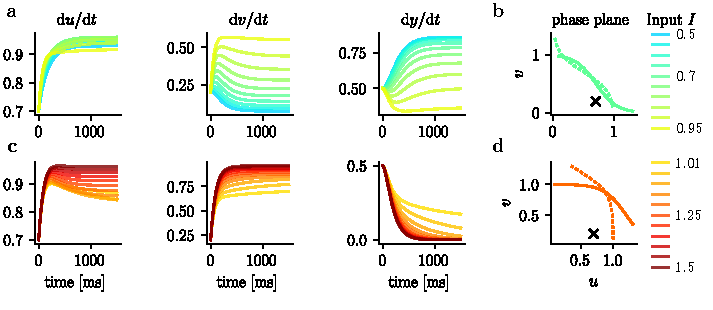
\includegraphics{figures/supp_regimes.pdf}
	\caption{\textbf{Comparison of dynamics in the intermediate and high input regime.} 
	\textbf{(a)} Evolution of $u, v$ and $y$ over time for different inputs from 0.5 to 0.95 in the intermediate input regime. Activity in $y$ shows a ramping-up activity. The activity of $y$ evolves to different steady states depending on the input. 
	\textbf{(b)}  The phase plane in the intermediate input regime shows two stable and one unstable fixed point. The nullclines of u (dashed) and v (solid) are shifted to higher activities when the input I is increased. The plot shows nullclines corresponding to an input of 0.7 and the black marker indicates the initial condition of dynamics in (a).
	\textbf{(c)} Same as (a) for the high input regime with inputs from 1.01 to 1.5. Activity in $y$ shows a ramping-down activity, converging to 0 independent of input.
	\textbf{(d)} Same as (b) for high input regime.  The phase plane in the high input
	regime shows one stable fixed point. The nullclines of u (dashed) and v (solid) are
	shifted to lower activities when the input $I$ is increased. The plot shows nullclines corresponding to an input of 1.2 and the black marker indicates the initial condition of dynamics in (c).
	}
\label{regimes}
\end{figure}

\subsection{Experiment Simulation in the High Input Regime}
To simulate time reproduction experiments in the high input regime, the following changes must be made. 
The threshold was set to a value lower than 0 (e.g. 0.1) and initial $I$ was increased to a value above 1 ($I_0 = 1.02$). The reset impulse after each epoch had to be stronger by a factor of 10 and with opposite sign to bring the activity in $y$ back to a higher level.

\begin{equation} \label{EqhighI}
	\begin{split}
	\tau\frac{\text{d}u}{\text{d}t} & = -u + \theta(W_{uI}I - W_{uv}v + \eta_u + 10*I_r) \;,\\
	\tau\frac{\text{d}v}{\text{d}t} & = -v + \theta(W_{vI}I - W_{vu}v + \eta_v - 10*I_r) \;.\\
	\end{split}
\end{equation}

There is no need to change the update mechanism, even though the relation of the input $I$ and the slope is reversed. This is because $y$ approaches the threshold from above and not from below, so the relation of $y$ and $y_{\text{th}}$ is reversed and the update of $I$ is correct. 

The noise was set to the same value as in simulations in the intermediate regime ($\sigma$ = 0.02). The standard deviations increased linearly. For increasing $\sigma$ the standard deviation drops slightly and then plateaus for $\sigma$ larger than 0.1. The CV has similar values as in the intermediate regime with 0.13 for the short and 0.12 for the long range for a $\sigma$ of 0.02 (Supplementary Fig. \ref{sup:highI}a). 
An example of the experiment dynamics for four consecutive simuli is displayed in Fig. \ref{highI}a.

\subsection{Error-Minimizing Parameters in the High Input Regime}
Just as for the intermediate input regime, optimized parameter $K$ and $\tau$ were found that minimize the MSE of reproductions. 
Again, the model is able to produce biologically plausible slopes for most time constants. 
Across all $\tau$ larger 40~ms, optimal $K$ is smaller for the long range compared to the short range.
The MSE is minimal for $\tau* = 60$~ms for both the short and the long range, with $K* = 4$ and $K* = 2.5$  for the short and the long range, respectively. Optimal $\tau*$ and $K*$ result in a biologically plausible slope only for the long range (slope of 0.68). For the short range the slope is too flat (slope of 0.74).
Behavioral results of experiment simulation with error-minimizing parameters show a regression to the mean. In contrast to the intermediate input regime, standard deviations of the reproductions do not grow linearly in the long range (Fig. \ref{highI}b).
For dynamics of $y$ over the whole experiment see Supplementary Fig. \ref{sup:experiment_high}.

\begin{figure}[ht]
	\centering
	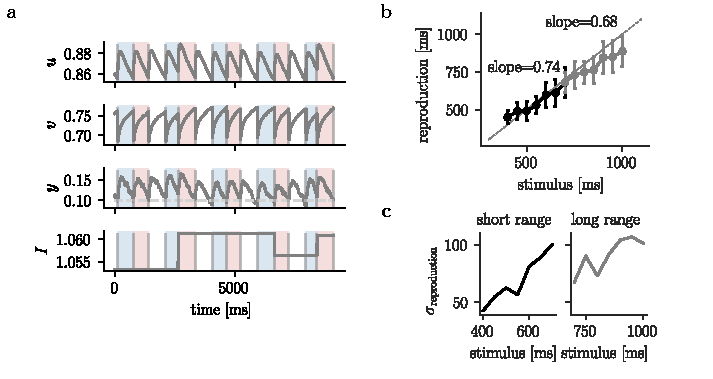
\includegraphics{figures/highI.pdf}
	\caption{\textbf{Experiment Simulation in the High Input Regime.} 
	\textbf{(a)} Activity of $u, v, y$ and $I$ for five example stimulus intervals of 650, 500, 600, 700, 450 ms. Stimulus presentation and reproduction epochs are highlighted in blue and red, respectively. The delay period between trials is shown in white. Initial values are set to $u_0=0.8 , v_0=0.6 , y_0=0.1, I_0=1.04$ and the threshold $y_{\text{th}}$ is set to 0.1. 
	\textbf{(b)} Top: Mean reproductions for simulation with 500 trials for each stimulation with the short (black) and long (gray) stimulus range. The value of $K$ is optimized to minimize errors in reproductions for a time constant of $\tau = 60$ ms. For the simulation with short stimulus range optimal $K$ was 4, with the long stimulus range optimal $K$ was 2.5.
		The slope is the result of a linear regression between stimuli and reproductions.
		Bottom: Standard deviation of reproductions for each stimulus for the short and long range from the simulation in (b).
	}
\label{highI}
\end{figure}

\subsection{Comparison of Experiment Simulations}
The results of simulations with optimal parameter combinations were used to compare the simulations in the intermediate and high input regimes.
Their behavioral results are displayed in Fig. \ref{fig:parameter}c for the intermediate and Fig. \ref{highI}b for the high input regime.
The mean input $I$ for each stimulus shows an almost linear increase (or decrease for the high input regime) within a range. The increase (or decrease) is shallower for the long range due to the lower $K*$ used in the simulation (Fig. \ref{fig:comparison}b, d).
The maximum and minimum input $I$ during the simulation for the short or the long range were used to examine the most distant nullclines of $u$ and $v$ in the phase plane(Fig. \ref{fig:comparison}a, c). 
In the intermediate regime, the difference between maximal and minimal $I$ is larger and the nullclines are also farther apart.


\begin{figure}[!htb]
	\centering
	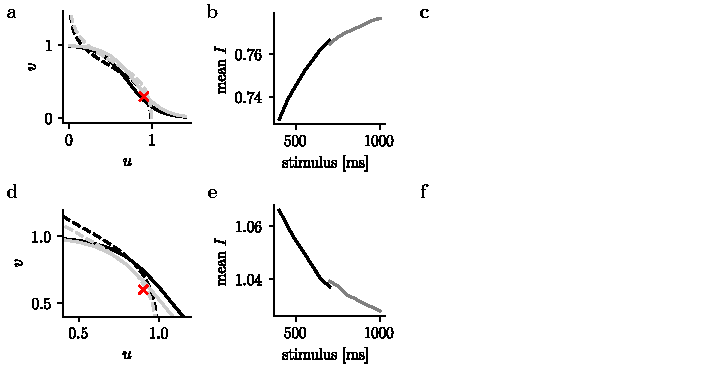
\includegraphics{figures/supp_comparison.pdf}
	\caption{\textbf{Comparison of experiment simulations.}
	\textbf{(a)} The phase plane in the intermediate input regime shows two stable (blue) and one unstable (light blue) fixed point. The nullclines of $u$ (dashed) and $v$ (solid) are displayed. Black and gray nullclines correspond to an input of 0.71 and 0.79, respectively, which corresponds to the maximal and minimal input in the experiment simulation for the short and long range in Fig. \ref{fig:parameter}c.
	\textbf{(b)} Mean input during the reproduction epoch for each stimulus of the short (black) and long (gray) range for the experiment simulation in the intermediate input regime with optimized parameters from Fig. \ref{fig:parameter}c.
	\textbf{(c)} The phase plane in the high input regime shows one stable (blue) fixed point. The nullclines of $u$ (dashed) and $v$ (solid) are displayed. Black and gray nullclines correspond to an input of 1.081 and 1.017, respectively, which corresponds to the maximal in minimal input in the experiment simulation for both the short and long range in Fig. \ref{highI}b.
	\textbf{(d)} Same as (b) for the experiment simulation in the high input regime with optimized parameters from Fig. \ref{highI}b.
	}
\label{fig:comparison}
\end{figure}

\section{General Underestimation}
%motivate why interesting
For a regression to the mean the indifference point of a linear regression between stimuli and reproductions should correspond to the mean of the stimulus range (550~ms for the short and 850~ms for the long range).
The indifference point (for behavioral results in Fig. \ref{fig:parameter}c) is 595~ms for the short range and 710~ms for the long range. Thus, in the long range simuli are in general underestimated. 
The same is the case for the high input regime (\ref{highI}b).
What is the reason for the general underestimation of larger inputs? 
It is not uncommon for stimuli in larger ranges to be generally underestimated in magnitude estimation across time domains. Time reproduction experiments with gerbils and humans show a general underestimation across ranges (Fig. \ref{fig:underestimation}a, \cite{Henke2022}). 
The cause has not yet been researched and could be due to many reasons ranging from lapsing attention to impatience. 
It is necessary to investigate whether the underestimation in the model's behavioral output is caused by the regime in which the model operates, or whether it is a phenomenon that arises from optimal choice of parameters.
Possible parameters of the model that could influence the behavior are the delay period between trials, the fixed threshold and the common time constant between stimulus ranges. 

\subsection{Delay Period Influences Reproductions}
The simulations were performed with a common time constant $\tau$ that was set between the optimal $\tau*$ for the short and long range, respectively.
General underestimation in simulations with the long range can be compensated by increasing the time constant towards the optimum of the long range. However, this causes a general overestimation in the simulation with the short range (Supplementary Fig. \ref{sup:othererror}b). 
Thus, a common time constant $\tau$ contributes to the under- and overestimation of stimuli, when it's too far from the range's optimum. But even at the optimum, simulations show a slight general underestimation in the long range.
Hence, there are several causes for this problem.

Another observation is that for both the long and short range, the best reproductions were obtained for stimuli near to 700~ms.
Following this observation, we simulated an experiment with a stimulus range that was situated around 700~ms (550, 600, 650, 700, 750, 800, 850 ms). 
The mean of 700~ms corresponds to the maximum of the short range and the minimum of the long range, and also complies with the length of the fixed delay period between trials.
In Fig. \ref{fig:delay}a the behavioral results show regression to the mean with a slope of 0.82 and an indifference point of 657~ms.
When setting the delay period at the maximum of the long range instead (1000 ms), a general overestimation of stimuli from the short range occurs (Supplementary Fig. \ref{sup:delay}c).
This led to the assumption that a delay period too far from the range's mean leads to under- or overestimation. 
A comparatively short delay period compared to the mean of stimuli leads to distorted updates, because $y$ cannot reach threshold value in the short time period with mean $I$. 
After resetting, the following measurement period is started from lower values in $y$. 
Setting the delay period equal to the mean of the short or long range 
eradicates general underestimation (Supplementary Fig. \ref{sup:delay}a, b).
In the high input regime, adapting the delay period does not resolve the general underestimation. Thus, only the intermediate input regime is used in the following analysis.

\subsection{Adjusted Experiment Simulation}
The previous analysis showed, that there are two main problems that caused distorted stimulus reproductions. 
First, a common time constant between experiments with different ranges skews the reproductions.
Second, is a hyperparameter of the experimental design affecting the reproductions. The delay period between trials should not influence reproductions.
Since the time constant in the model can be interpreted as a rate time constant, it is justifiable to adapt it between experiment with different stimulus ranges. 
This would correspond to a firing rate adjustment in the population to an experimental setting.
In a biological system, an inhibitory population could scale the rate time constant according to the stimulus statistics.
%todo: K not comparable across ranges (not smaller for long range etc)
Furthermore, the model needs to be adjusted to take into account the impact of the delay period on the reproductions. 
% delay=mean of range
Setting the delay time to the mean of the stimulus range used in the simulation doesn't make sense from a design perspective. It should be possible to choose the delay period between trials arbitrarily and independently of the stimulus range. 
% long delay + separate tau
Similarly, the delay period could be chosen long enough to allow the system to evolve to a steady state. However, this would mean that the delay time cannot be chosen independently.
% no delay
Another way to solve the problem of the delay epoch, is to neglect the delay in the simulation of the experiment (Fig. \ref{fig:delay}b).
The reproduction period always ends when the threshold $y_\text{th}$ is met. If the measurement period of the subsequent trial follows directly after it, it always starts at the same value of $y$. 
This does not necessarily mean, that the experimental design is limited. When simulating experiments that include a delay period between trials or even between measurement and reproduction epoch, it can be assumed that information is stored in the system until the beginning of the next epoch. 
In neural networks, it has been shown that the timing information in the state space can be held over a delay time (\cite{Bi2020}).
Neglecting the delay epoch in combination with independent $\tau*$ for each range leads to characteristic effect and biologically plausible slopes (Fig. \ref{fig:delay}c).
% reset on fixed value
% learn I for delay
Solutions that incorporate a delay period into the simulation itself would require model adjustments.
Either the reset is changed from an impulse to a fixed reset value, or the input is updated separately during the delay epoch based on an error to always reach the threshold. 

Unless otherwise specified, error-minimizing $\tau*$ and a delay of 0~ms are used for each stimulus range in following simulations. The regime of $I$ remains similar to previous simulations with delay and common $\tau$. There is an overlap in $I$ and $K$ is no longer comparable due to separate $\tau$ between different ranges (Fig. \ref{fig:new_ranges}b).

\begin{figure}[ht]
	\centering
	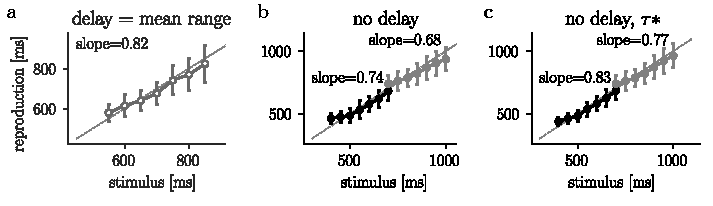
\includegraphics{figures/delay.pdf}
	\caption{\textbf{Behavioral results with altered delay.} 
	\textbf{(a)} Behavioral results of an experiment simulation with the previously utilized delay of 700 ms. The stimulus range that was used to sample stimuli from has a mean equal to the delay of 700 ms. The time constant and update parameter were both optimized based on the MSE ($\tau$ = 170 ms, $K$ = 17.5). Other parameters like threshold and initial values were not changed. 
	\textbf{(b)} The delay period was set to 0 ms in simulations with the short and long range (black and gray, respectively). The time constant was set to 165 ms, which corresponds to the mean of the optimal $\tau$ for the short (130 ms) and long (200 ms) range. For $\tau$ = 165 ms, the update parameter $K$ was optimized (short range $K$ = 21, long range $K$ = 13). Note different axes of figures in (a) and (b).
	\textbf{(c)} Same as (b) but with independent, optimal time constant. For the short range $\tau*$ = 130, $K$ = 14 and for the long range $\tau*$ = 200, $K$ = 20.
	}
\label{fig:delay}
\end{figure}


\section{Influence of External Variability on Behavior} \label{externalvar}
Regression to the mean depends on the discrimination abilities of the individual subject. In the model, this is reflected by internal noise $\sigma$.
In addition, variability of the environment affects the behavior, which is captured by the statistics of stimuli over the course of an experiment. 
When internal noise is fixed, the external variability can be modified independently. 
The effect of external variability on the update parameter can be investigated by modifying the mean or the variance of stimuli. 

\subsection{Effects of Stimulus Statistics in Real Behavior}
With larger time intervals, internal estimates get noisier and regression of reproductions gets stronger. This is well described by the \textit{range effect} across species (\cite{Cicchini2012}, \cite{Henke2021}, \cite{Henke2022}, \cite{Sohn2019}). 
Besides the mean, also the variance of stimuli could influence the reproduction.
Larger variance can be achieved by reducing the sampling frequency of the stimulus range or by expanding the width of the range, accommodating more distance time intervals. 
The effect of changing the variance of stimuli on the behavior has not been well studied.
%%%%%%%%%%%%%%%%%%%%%%%%%%%%%%%%%
There are three different effects that greater variance could have on behavior. 
Reproductions could improve, leading to a weaker regression. This would mean that subjects rely less on the prior. 
Intuitively, larger variance means that differences of time intervals get more apparent and discrimination becomes easier (e.g. stimuli are further apart or extremes are more distinct). 
This scenario is predicted by a model that uses noisy integrators linked by an adaptive reference in \cite{Thurley2016}.
On the other hand, a change in variance might have no effect on behavior, if the mean is fixed. According to this, only the mean value would have an influence on the reproduction performance.
This seems to be the case in \cite{Petzschner2012}, since performance of the range with larger variance doesn't get better. 
Finally, reproductions be worse with greater variance. This was demonstrated in the case of sound intensity estimations by \cite{Teghtsoonian78}.
In most studies that included experimental data with varying variance of stimuli, the effects on regression were not examined. 

\subsection{Optimality Predicts Regression Effect and Range Effect}
To test the behavior of the model with respect to the external variability of stimuli, additional ranges were used, differing in mean, width and sampling frequency.
The short and the long range include seven stimuli spanning 300 ms, with mean values of 550 and 850~ms, respectively. 
Two ranges had the same variance and width, but shifted mean values at 700~ms (mid range) and 1050~ms (extra-long range). With increasing mean, the range effect predicts a flatter slope. 
In addition, ranges were examined whose mean was equal to one of the ranges above, but which had a higher variance.
Including all stimuli from the short and the long range, the all range has the same mean as the mid range, but a larger width (600 ms) and therefore higher variance.
The short-few and all-few range encompasses the short and the all range, respectively, but with smaller number of stimuli, the variance increases in both cases 
(Fig. \ref{fig:new_ranges}a, Supplementary Fig. \ref{sup:ranges}c).
%%%%%%%%%%%%%%%%%%%%%%%%
%Optimal $\tau*$ for stimulus ranges are as follows: short~130~ms, mid~170~ms, long~200~ms, extra-long~230~ms, all~150~ms, ~short-few~120~ms and all-few~160~ms.
For all ranges, the slope of the linear regression between stimuli and reproductions is below one. Thus, simulations with error-minimizing parameters predict the regression effect across several ranges. 
The slopes decrease significantly as the mean of the stimulus range increases, except for the short and mid range (Fig. \ref{fig:new_ranges}c).
Thus, the model predicts the range effect only for sufficiently large changes in the mean. 
(Kolmogorov–Smirnov two-sample test, p$<$0.01, n=21 for each distribution, Bonferroni correction for multiple testing).
Across ranges that only change their mean value (short, mid, long and extralong), the slope has a linear correlation with the mean value of the range (Pearson correlation r=-0.95, $p<0.05$).

When the experiment was simulated with a common $\tau$ of 165~ms between ranges, $K*$ is significantly lower for the mid range (16.71) compared to the short range (21.33), but slopes show no significant difference (Supplementary Fig. \ref{sup:ranges}a, b).
Decreasing $K*$ for increasing mean of ranges is captured by the model beyond the short and the long range.
(Kolmogorov–Smirnov two-sample test, n=20 for each distribution, p$<$0.01, Bonferroni correction for multiple testing).\\

%%%%%%%%%%%%%%%%%%%%%%%%%Grenzen des Models%%%%%%%%%%%%%%%%%%%%%%%%%%%%%%%
%underestimation extra long: grenzen des Models, breaks down
%reason for range effect
\noindent What causes the range effect in the circuit model?
The model is situated in a dynamic regime, that displays time reproductions close to real behavior.
Error-minimizing parameters predict the regression and range effect across multiple stimulus ranges.
Decreasing slopes for larger stimulus ranges occur because they approach the limit of the dynamic regime (Fig. \ref{fig:new_ranges}b).
When the stimulus ranges are pushed to more extreme values, the behavior of the model breaks down. Reasons for a breakdown of the behavior are a too large number of timeouts in the case too short time intervals. If time intervals are too, the variance in reproductions increases sharply and $K$ is pushed to lower values, resulting in slopes that are outside the observed behavior. 
This means that the regime of the model has to be adapted to major changes in the external statistics. 

\subsection{Optimality Predicts no Effect of Variance on Behavior}
How does the slope change when the mean of stimuli remains constant, but variance is increased?
The statistics of stimuli can be summarized by the ratio of the mean and variance of the stimulus range: $\frac{\text{E(t)}}{\text{var(t)}}$.
Higher variance in ranges with lower stimulus sampling (short-few, all-few) shows no significant difference from their counterparts with normal stimulus sampling (short, all).
Furthermore, a larger width of stimuli does not result in a significant larger or smaller slope (all range vs mid range).
Therefore, increasing variance is not affecting the reproduction of stimuli in the model.
(Kolmogorov–Smirnov two-sample test, n=21 for each distribution, Bonferroni correction for multiple testing).
Considering only the mean, there is a significant correlation with the slope (Pearson correlation r=-0.96, $p<0.001$), but not with the external variability ratio (Pearson correlation r=-0.65, $p=0.12$) (Fig. \ref{fig:new_ranges}c).
In the simulation with a common $\tau$ there is no significant difference in $K*$ when the variance is changed (Supplementary Fig. \ref{sup:ranges}a, b).
However, increasing the variance of a range leads to a significant increase in MSE in all cases (Fig. \ref{fig:new_ranges}d).  
(Kolmogorov–Smirnov two-sample test, n=21 for each distribution, p$<$0.01, Bonferroni correction for multiple testing).

\begin{figure}[ht]
	\centering
	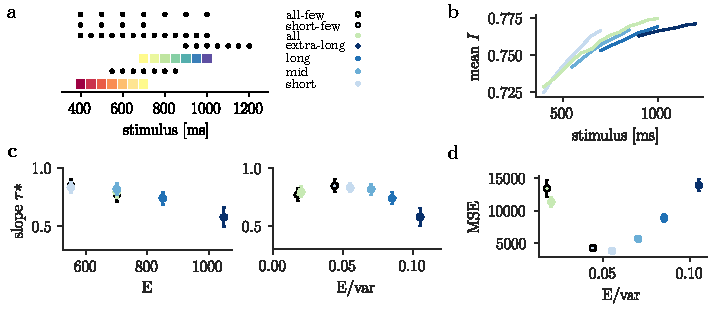
\includegraphics{figures/ranges_new2.pdf}
	\caption{\textbf{Behavioral slopes with varying stimulus statistics.} 
	\textbf{(a)} Parameter simulations were performed with stimulus ranges that differed in mean and variance to the short and long range. The mid range has its mean at the overlap of the short and long range. The extra-long range has its mean above the long range. Both the mid and extra-long range have the same number of stimuli as the long and short range (7). To change the variance a range with more stimuli (13) that spans the short and long range was included (all range). Both the short and the all range were for the short-few and all-few range under sampled.
	\textbf{(b)} Simulations were performed with optimized $\tau*$ (and corresponding  $K*$): short 130 ms (14), mid 170 ms (17), long 200 ms (20), extra-long 230 ms (18), all 150 ms (14). Mean input $I$ for each stimulus was calculated for stimulation with different ranges. Colors correspond to legend in (a). 
	%short-few 120 ms (12) and all-few 160 ms (15)
	\textbf{(c)} Left: Slopes of behavioral results plotted against the mean of the range that was used. The error bars indicate standard deviation in the slope for different initialization. Colors correspond to legend in (a).
	Right: Slopes plotted against the ratio of the mean and the variance of each range. 
	\textbf{(d)} The MSE for simulations with error-minimizing parameters, plotted against the ratio of mean and variance of the range.
	}
\label{fig:new_ranges}
\end{figure}

\subsection{Comparison of Behavioral Output of Model to Real Data}
The circuit model predicts that a change in variance affects the MSE of the reproductions.
It also predicts, that only the mean and not the variance has an effect on the regression of reproductions, which is in contrasnt to the noisy integrator model proposed by \cite{Thurley2016}.
In the following section, we compare predictions of the model with behavioral data from time reproduction experiments with gerbils and humans. The stimuli in these experiments were several seconds long and came from either a short, mid, long or all range (data by Henke and Thurley).

Behavior in gebrils exhibits a regression effect for all ranges and a range effect for ranges with increasing mean. 
The variation in slopes between gebrils is considerably larger when the variance is increased.
At the individual level, both consistent and increasing performance with increasing variance is observed. 
There are three gebrils that show a linear increase in performance with decreasing ratio of the mean and variance of the stimulus range (Fig. \ref{fig:underestimation}b). The remaining four gerbils however, show no effect of variance on reproductions (Supplementary Fig. \ref{sup:underestimation}a).
On average Person correlation shows a significant linear relation of the slope with the mean (r=-0.62, $p<0.001$) and ratio of mean and variance (r=-0.61, $p<0.001$) in gerbils.
This correlation gets stronger when the all range is excluded (r=-0.75, $p<0.001$).
In humans, behavior is heterogeneous, and there is no range effect on average, but there is in some individuals (Fig. \ref{fig:underestimation}). There is no significant correlations of the slope with the mean or external variability ratio.
The root MSE increases as the variance increases across all subjects (Supplementary Fig. \ref{sup:underestimation}b).

%%%%%%%%%%%%%%%%%%%%%%%%%% comparison
The circuit model predicted no effect of variance on the regression, but on the error in reproductions. 
Gebrils show a discrepancy in performance when variance is increased. 
The model captures only one possible behavior, namely not taking into account a change in variance. 
There is no significant correlation of the slope with the external variability ratio in the model, when in gerbils there is.
However, the model predicts correctly increasing error in reproductions with higher variance (Fig. \ref{fig:new_ranges}b).


%EVAR all:    g r=-0.61, $p<0.001$, h r=-0.05, $p=0.802$, m r=-0.64 $p=0.12$
%E all:       g r=-0.62, $p<0.001$, h r=-0.08, $p=0.718$, m r=-0.96, $p<0.001$
%EVAR(E) sml: g r=-0.75, $p<0.001$, h r=-0.4, ???       , m r=-0.95, $p<0.05$

\begin{figure}[ht]
	\centering
	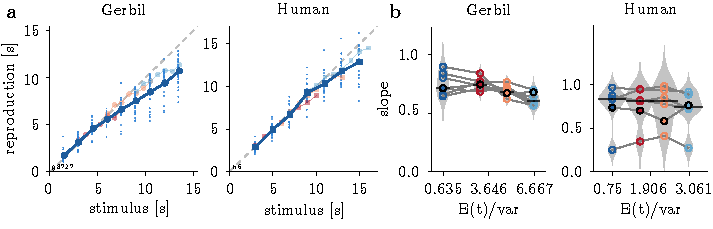
\includegraphics{figures/underestimation.pdf}
	\caption{\textbf{Effects of stimuli statistics on behavior of gerbils and humans.}
	\textbf{(a)} Representative behavioral results of time reproduction of a gerbil (left) and a human (right). Stimuli were several seconds long. Four experiments were conducted with different ranges: short (red), mid (orange), long (light blue) and all (blue). Large markers display the mean of trials. Small dots show reproductions of single trials for the experiment with the all range.
	Ranges differed slightly between experiments with gerbils and humans. 
	\textbf{(b)} Slope of the linear regression between stimuli and reproductions for seven gerbils (left) and six humans (right) plotted against the ratio of the mean and variance of the stimulus ranges. Vertical black markers indicate the median of slopes and gray violin plots illustrate the distribution over all animals. Slopes for different stimulus ranges of one animal are connected by lines. 
	Figure courtesy of Kay Thurley and Josephine Henke.
	}
\label{fig:underestimation}
\end{figure}

%%%%%%%%%%%%%%%%%%%%%%%%%%%%%%%%%%%%%%%%%%
\section{Discussion}
It has been shown...
Here, we extended the model and showed that...
model different approch
% in general models of time reproduction Einordung
%relate to Bayes (statistical model different approach)
%optimization and error minimizatoin

%what is the prediction of the model? what dies the data say? 
% there is remapping zwischen ms und s in real data, millisecond to seconds, adaptation due to same effects observed. 
% no remapping in model
% some gebrils are adapting regime others are not when var is increased


This means, when using the model in experiments with even shorter or longer time intervals, the regime of the model has to be adjusted. 
A sort of adjustment also happens in real behavior. This becomes apparent when comparing the regression between experiments conducted in different time domains, e.g. milliseconds vs. seconds. There is no much stronger regression in the second range compared to the millisecond range. Qualitatively the regression and range effect look the same for different stimulus ranges in both time domains (\cite{Jazayeri2010}, \cite{Henke2021}). 

%experiment suggestion: inclunece of var graduatly, when remapping? more expreme changes, other chages like sampling? how does the discrepencey arises?

%generalization to other modalities critique: metric to code different types of magnitudes. \cite{VanOpstal2013}

\pagebreak
%Shifting the threshold to higher or lower values of $y$ does not resolve under- or overestimation. However, the threshold has to be set in an appropriate scope to avoid exceeding timeouts. 

\setcounter{section}{0}
\addcontentsline{toc}{section}{Supplements}
\section*{Supplements}
\setcounter{figure}{0}
\setcounter{table}{0}
\setcounter{equation}{0} 
\renewcommand{\figurename}{Supplementary Figure}
\renewcommand{\tablename}{Supplementary Table}

\section{Methods}
\subsection*{Circuit}
For simulating the dynamics of $u, v, y$ and $I$ Euler's method was used with a step size $\Delta t$ set to 10 ms.
The reset mechanism of $u$ and $v$ is switched on for one time step after every epoch and the update mechanism of $I$ is switched on for one time step after the measurement epoch only.
Noise is independently sampled for every time step from a Gaussian distribution with standard deviation $\sigma$.

\subsection*{Timeouts}
Reproductions that do not reach the threshold in a certain time span (twice the stimulus interval) are classified as timeout trials. 
If the threshold is crossed particularly early, the trial is also classified as (early) timeout trial (crossing before 0.2 of stimulus interval).
Simulations that exceed a fixed number of timeout trials (10\% of all trials in the experiment) were excluded from analysis.
If timeout trials occurred for a single stimulus more than 10\% of all trials of this stimulus, the simulation was also discharged.
For different parameter combinations, the number of timeouts were exceeded (a combination of too small $\tau$ and too high $K$).


\subsection*{Experiment Simulation}
In all simulations in the intermediate regime, the threshold $y_\text{th}$ was set to 0.7. The model worked with higher and lower thresholds robustly.  
For experiment simulations with 500 trials, the increase of the standard deviation of reproductions plateaus with noise levels $\sigma > 0.1$. This was tested with parameters set to $\tau=100$, $K_\text{short}=8.5$ and $K_\text{long}=6$.
The standard deviation of reproductions grows monotonically for increasing stimulus intervals for tested noise levels (Supplementary Fig. \ref{sup:CV}b).
Further, the coefficient of variation (CV) was used to quantify the degree of variation. It is defined as $\text{CV}=\frac{\sigma_\text{reproduction}}{\mu}$ for each stimulus, where $\mu$ corresponds to the stimulus interval and $\sigma_\text{reproduction}$ to the standard deviation of the corresponding reproductions. 
To achieve variations close to real data, reproductions should have a CV of 0.2 to 0.4 that is constant over all stimulus intervals (Supplementary Fig. \ref{sup:CV}c).
For all simulations the noise level $\sigma$ was set to 0.02, where the mean CV for the short range was 0.1 and for the long range 0.15 with the parameters from above.

In all experiment simulations, a series of 500 trials was presented to the model.
Stimuli were randomly chosen from the short (400-700 ms) or the long (700-1000 ms) stimulus range (Supplementary Fig. \ref{sup:CV}a).
The stimulus series had a uniform distribution of stimuli, a repetition of all seven stimuli in every 20 trial windows and no remarkable oscillation.
To allow for optimization of $K$ the same stimulus series was used. Added noise was initialized equally to extract changes in results only based on parameter changes.
Different noise initialization influence the optimal value of $K$ slightly. For 20 simulations with $\tau=140$ and $\sigma=0.02$ the mean optimal $K$ and standard deviation for the short range were $K = 14.45$, std = 0.49 and for the long range $K = 9.91$, std = 0.77. 

\subsection*{Optimality by Minimizing MSE}
We minimized the error in the interval reproductions across the experiment, we defined the $\text{MSE} = \text{bias}^2+\text{var}$, with the bias specified as the squared difference between the mean reproduction $\bar{t_{r}}$ for each stimulus interval $t_s$ in the stimulus range $S$ and variance as mean $\sigma^2$ for all stimulus intervals in $S$.
\begin{equation} \label{MSE}
	\begin{split}
	 \text{bias} & = \frac{1}{S} \sum \limits_{i=1}^{S} (\bar{t_{r_i}} - t_{s_i}) \;,\\
	 \text{bias}^2 & = \frac{1}{S} \sum \limits_{i=1}^{S}(\bar{t_{r_i}} - t_{s_i})^2 \;,\\
	 \text{var} & = \frac{1}{S} \sum \limits_{i=1}^{S}(\sigma_i^2) \;.\\
	\end{split}
\end{equation}

\subsection*{Errors Minimization with Other Metrics}
Optimal values of $K$ are based on the MSE, which composed of the squared bias and the variance of reproductions. 
Time constants $\tau$ with the minimal MSE for a value of $K$ differ between the short and the long range. For the short range the optimal time constant $\tau = 120 ms$, for the long range $\tau = 200 ms$ (Supplementary Fig. \ref{sup:othererror}a, b). If optimization is based only on the squared bias, optimal time constants are 100 ms for the short and 110 ms for the long range. 
The variance is pushing the optimal time constant to lager values for both stimulus ranges. 
Similarly, optimal $K$ is pushed to lower values by the variance (Supplementary Fig. \ref{sup:othererror}c, d).
For all optimized values, be it on the squared bias, the variance or combined in the MSE, there is a general underestimation of stimulus intervals from the long range, which becomes appeared in Supplementary Fig. \ref{sup:othererror}e.

\subsection*{Statistical Analysis}
%If p-values are not provided, significance is indicated by * p<0.05, ** p< 0.01, *** p<0.001

\section{Supplementary Figures}
\begin{figure}[!htb]
	\centering
	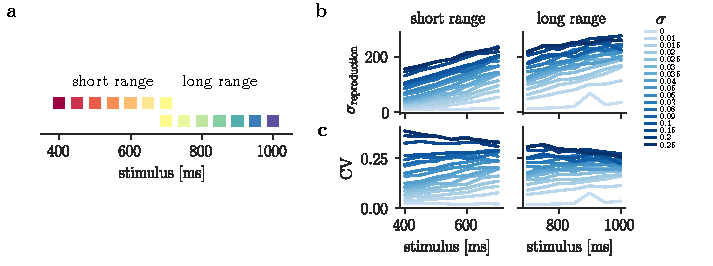
\includegraphics{figures/supp_CV.pdf}
	\caption{\textbf{Experiment description and noise levels.} 
	\textbf{(a)} The short and the long stimulus range comprised time intervals from 400 to 700 ms and 700 to 1000 ms, respectively.
	\textbf{(b)} Standard deviation of reproductions for each stimulus in an experiment simulation with 500 trials and $\tau=100$. $K$ was set to 8.5 and 6 for the short and long range respectively. 
	\textbf{(c)} Same as (a) but standard deviation of reproductions normalized by stimulus duration (CV).
	}
\label{sup:CV}
\end{figure}

\begin{figure}[!htb]
	\centering
	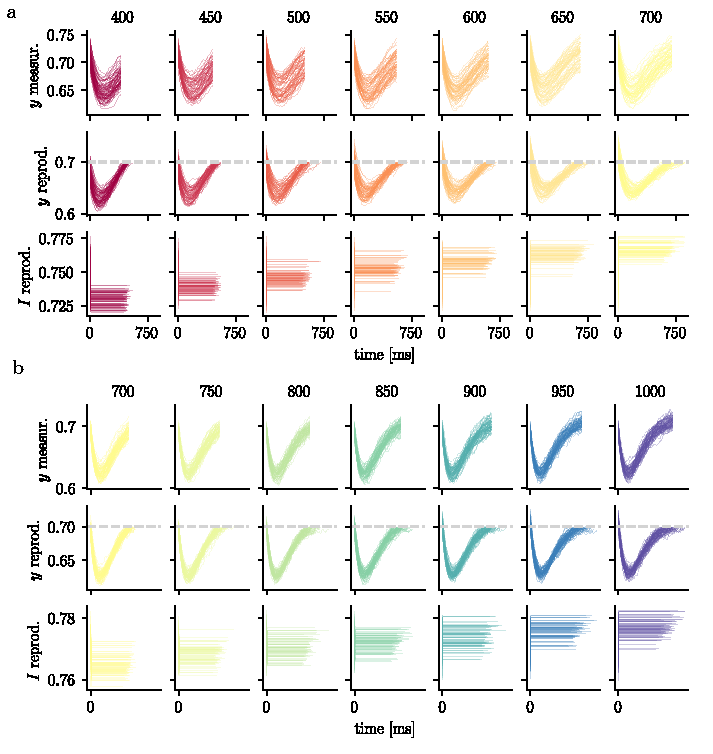
\includegraphics{figures/supp_experiment.pdf}
	\caption{\textbf{Experiment dynamics with optimized $K$.}
	\textbf{(a)} For an experiment simulation with 500 trials, a time constant $\tau$ of 130 and optimal $K = 13$, the activity was sorted according to epoch and stimulus interval. Stimuli were chosen from the short range. Upper row show the behavior of $y$ in the measurement epoch, middle row shows the behavior of $y$ in the reproduction epoch. The lower row shows the input level to the circuit during the reproduction epoch. 
	\textbf{(b)} Same as (a) with stimuli chosen from the long range and $K = 10$. 
	}
\label{sup:experiment}
\end{figure}

\begin{figure}[!htb]
	\centering
	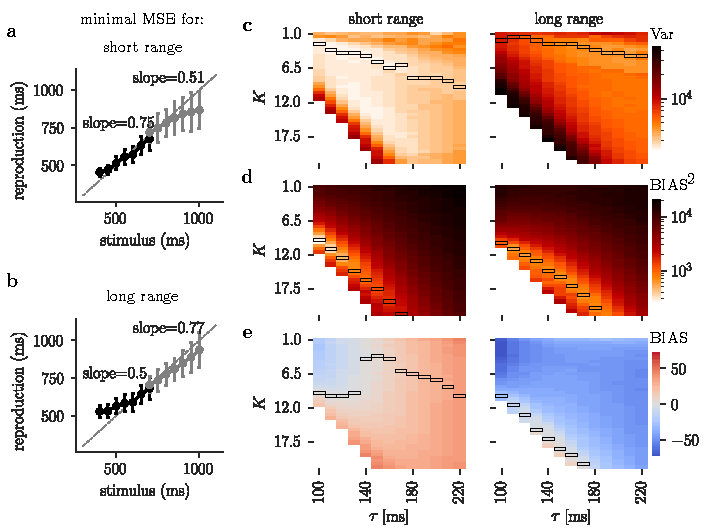
\includegraphics{figures/supp_othererror.pdf}
	\caption{\textbf{Extended parameter optimization.}
	\textbf{(a)} Behavioral results for a simulation with 500 trials, $\sigma = 0.02$ and optimized time constant $\tau$ for the short range ($\tau = 120$). For simulations with both short and long range, the optimal time constant for the short range was used. Optimal $K$ for $\tau = 120$ was 11 for the short, 7 for the long range.
	\textbf{(b)} Same as (b) with optimized $\tau$ for the long range ($\tau = 200$). Optimal $K$ for this time constant was 25 for the short range and 20 for the long range. 
	\textbf{(c)}  Simulations with 500 trials for each pair of memory parameter $K$, and $\tau$ at noise level $\sigma = 0.02$. Simulations were performed with stimuli chosen from the short (left) or long range (right). Color scale represents the variance of reproductions in the behavioral results. Minimal variance for each $\tau$ is encircled.
	\textbf{(d)} Same as (c), color scale represents the squared bias of reproductions. Minimal squared bias for each $\tau$ is encircled.
	\textbf{(e)} Same as (d), color scale represents the bias of reproductions. Values larger than 0 correspond to an overestimation, values smaller than 0 to an underestimation of the stimulus interval. Bias closest to 0 for each $\tau$ is encircled.
	}
\label{sup:othererror}
\end{figure}


\begin{figure}[!htb]
	\centering
	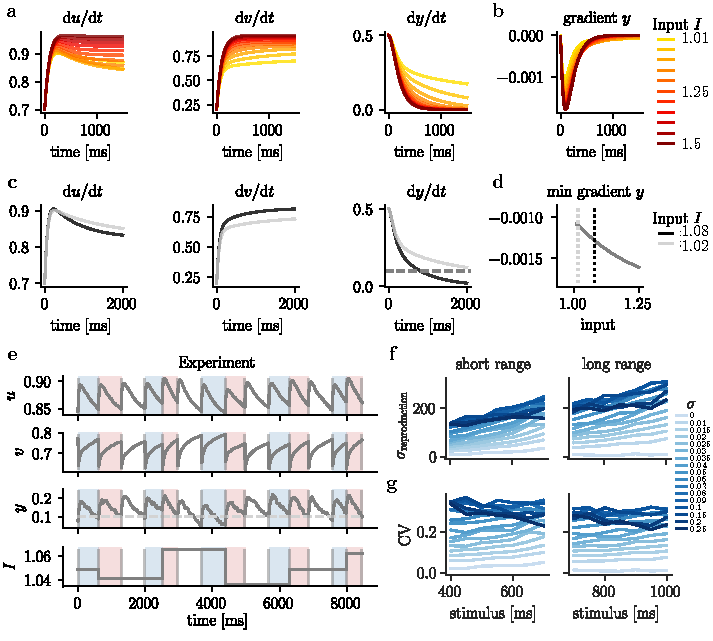
\includegraphics{figures/supp_highI.pdf}
	\caption{\textbf{Experiment description and parameter optimization in the high input regime.} 
	\textbf{(a)} Evaluation of noise for the high input regime of the model. Standard deviation (upper) and CV (lower) of reproductions for each stimulus in an experiment simulation with 500 trials and $\tau = 70$. K was set to 6 and 4 for the short and long range, respectively.
	\textbf{(b)} Simulations with 500 trials for each pair of memory parameter $K$ and time constant $\tau$ at noise level $\sigma$ = 0.02. Simulations were performed with stimuli chosen from the short (left) or long range (right). Color scale represents the slope of the linear fit between stimuli and reproductions. Behaviorally plausible slopes are encircled in blue and lie around 0.83 for the short and 0.73 for the long range. Empty spaces show simulations, that exceeded the number of timeout trials and where thus excluded from analysis.
	\textbf{(c)} Optimization of the memory parameter $K$ in the high input regime for different time constants $\tau$ at noise level $\sigma$ = 0.02. Color scale represents the MSE for an experiment stimulation with 500 trials for each pair of $K$ and $\tau$. Stimuli were either chosen from the short (left) or the long stimulus range. The minimal error for each $\tau$ is encircled in black and minimal error across all $\tau$ is additionally crossed. Parameter combinations that result in behavioral plausible slopes (b) are shaded in blue. 
	}
\label{sup:highI}
\end{figure}

\begin{figure}[!htb]
	\centering
	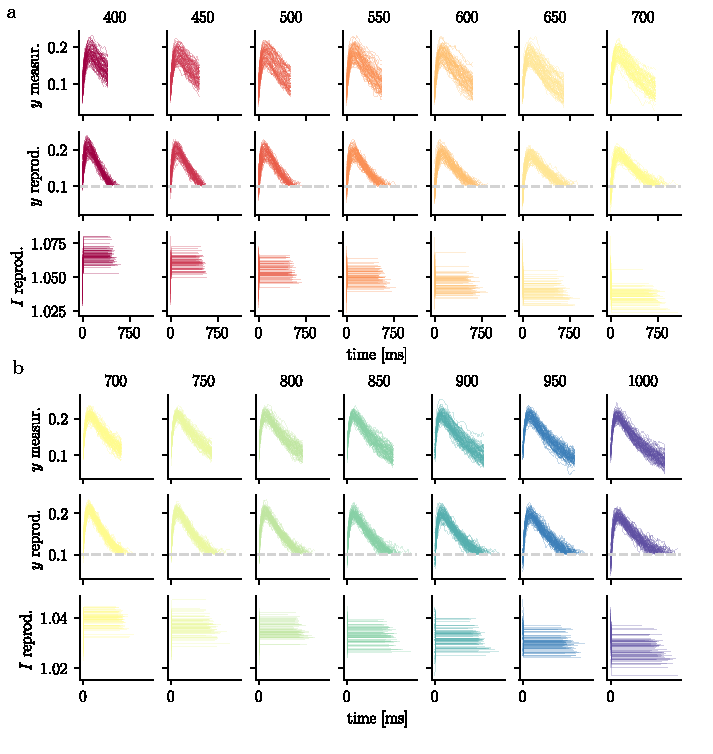
\includegraphics{figures/supp_experiment_high.pdf}
	\caption{\textbf{Experiment dynamics in the high input regime.} 
	\textbf{(a)} For an experiment simulation with 500 trials in the high input regime. The threshold is set to $y_{\text{th}}=0.1$ and $\sigma=0.02$. Parameters are set to optimized values with time constant $\tau = 60$ and $K = 4$. The activity was sorted according to epoch and stimulus interval. Stimuli were chosen from the short range. Upper row show the behavior of $y$ in the measurement epoch, middle row shows the behavior of $y$ in the reproduction epoch. The lower row shows the input level to the circuit during the reproduction epoch. 
	\textbf{(b)} Same as (a) with stimuli chosen from the long range and $K = 2.5$.
	}
\label{sup:experiment_high}
\end{figure}

\begin{figure}[!htb]
	\centering
	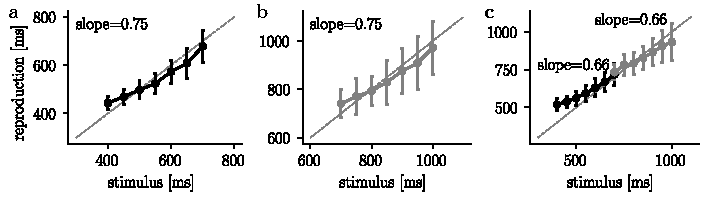
\includegraphics{figures/supp_delay.pdf}
	\caption{\textbf{Behavioral results with different delay periods.}
	\textbf{(a)} Behavioral results of an experiment simulation with stimuli of the short range and the delay period set to the mean of short range (550 ms). Time constant and update parameter are optimized based by minimizing the MSE ($\tau$ = 130, $K$ = 13). Other parameters like $\sigma$, threshold and initial values were not changed compared to previous simulations.
	\textbf{(b)} Same as (a) but for the long range with the delay period set to mean of the long range (850 ms). Optimized $\tau$ = 220 and $K$ = 22.
	\textbf{(c)} Behavioral results of experiment simulation with both the long and the short range and the delay period set to 1000 ms. The time constant is set 160 ms, which corresponds to the mean of the optimal $\tau$ for the short (110 ms) and long (210 ms) range. Optimal $K$ for the short ($K$ = 17) and long ($K$ = 11) range is optimized for the chosen time constant. 
	}
\label{sup:delay}
\end{figure}

\begin{figure}[!htb]
	\centering
	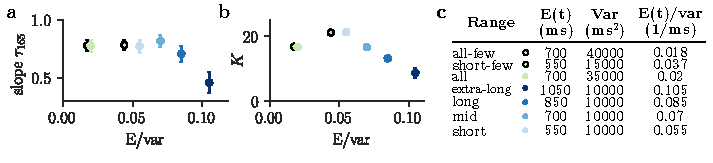
\includegraphics{figures/supp_ranges_new.pdf}
	\caption{\textbf{Influence of external variability on behavior with shared time constant.}
	\textbf{(a)} The slope of behavior resulting from experiment simulations with optimized $K$ for different ranges was determined and plotted against the ratio of mean and variance of the stimulus range. The time constant was set to 165~ms for all ranges, which corresponds to the mean of the optimal time constant of the short and long range. The error bars indicate standard deviation in the slope for different initialization. Colors correspond to the legend in (c). 
	\textbf{(b)} $K$ that minimized errors for a time constant of 165 ms for all ranges. 
	$K$ is plotted against the ratio mean and the variance of the stimulus range.
	The error bars indicate standard deviation in the slope for different initialization. 
	\textbf{(c)} Overview of all ranges used for simulations with their mean, variance and the ratio of both, that is used to characterize the ranges.
	}
\label{sup:ranges}
\end{figure}

\begin{figure}[!htb]
	\centering
	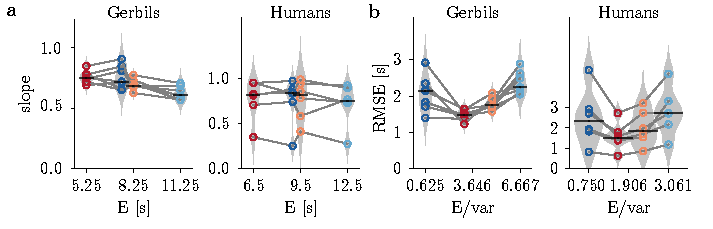
\includegraphics{figures/supp_underestimationE.pdf}
	\caption{\textbf{Effects of stimuli statistics on behavior of gerbils and humans.}
	\textbf{(a)} Slope of the linear regression between stimuli and reproductions for seven gerbils (left) and six humans (right) plotted against the mean of the stimulus ranges. Vertical black markers indicate the median of slopes and gray violin plots illustrate the distribution over all animals. Slopes for different stimulus ranges of one animal are connected by lines. Note that ranges short (red), mid (orange), long (light blue) and all (blue) differed slightly between experiments with gerbils and humans.
	\textbf{(b)} xxx
	Figure courtesy of Kay Thurley and Josephine Henke.
	}
\label{sup:underestimation}
\end{figure}

\pagebreak

\section{Design}
The code is designed in a modular way, such that multiple types of experimental procedures with shared functionality are accessing the same basic circuit, which is implemented in \texttt{BaseSimulation} as shown in Figure \ref{fig:code}.
The implementation of the basic circuit can be reused for all epochs.
Different experiments can have different result types, all of which can be found in \texttt{result.py}. After each experiment, the results are gathered and stored together, consisting of the parameter set, the simulation time course, a list of reset time points, a list of production times, a list of indices of timeout trials and the stimulus list.
Analysis of the results is performed in the same file. Depending on the analysis (e.g. behavioral), different plots are implemented in \texttt{plot.py} to visualize the results. 

All parameters are set and described in \texttt{Params} and can be modified individually or by reading a parameter dictionary. The parameters configure the circuit. 
To initiate a simulation, the parameter set is handed to one of the implemented experiments. 
An interval reproduction experiment, as described in this report is implemented in \texttt{experiment\_simulation.py}. 
Parallel simulations of one trial (one delay, measurement and reproduction epoch) is implemented in \texttt{parallel\_simulation.py}.
Both \texttt{experiment\_simulation.py} and \texttt{parallel\_simulation.py} contain a simulate function that accesses the base simulation (\texttt{BaseSimulation}) with the implementation of the basic circuit.
For each epoch or update/reset step, the simulate function feeds the according time steps and initial conditions into the network in \texttt{BaseSimulation}. Depending on the epoch, the reset and update mechanism are tuned on or off. 
After each epoch or pulse, the results of the network are joint to the time course of the experiment in trial\_update. The simulate function returns a \texttt{SimulationResult} or \texttt{RangeParallelSimulationResult} object.

For an overview of the code structure see Figure \ref{fig:code} and for its usage see simulations.ipynb at \href{https://github.com/KatharinaBracher/MScThesis}{github.com/KatharinaBracher/MScThesis}. 

\section{Implementation}
All simulations and analysis were performed with Python 3.9.7. 
The following libraries were used: matplotlib (3.5.1), NumPy (1.22.3), SciPy (1.8.0), scikit-learn (1.0.2). 
An experiment simulation can not be parallelized, since each step depends on the previous one.
% For the parameter search multiple experiment simulations were parallelized 

% server

\begin{figure}[ht]
	\vspace*{-2cm}
	\makebox[\textwidth][c]{\includegraphics[width=1.2\textwidth]{figures/codeStructure.drawio.pdf}}
	\caption{\textbf{Design.} The base simulation and different procedures (experiment, parallel) are all implemented in separate files. All results and analysis are collected in \texttt{result.py}, all plot for different result types are collected in \texttt{plot.py}}
\label{fig:code}
\end{figure}


\clearpage
\addcontentsline{toc}{section}{References}
\printbibliography




































\end{document}